% arara: pdflatex
% !arara: indent: {overwrite: yes}
\documentclass{beamer}
\usepackage[latin1]{inputenc}
\usetheme{CambridgeUS}
\usecolortheme{dolphin}
\usepackage{standalone}
\usepackage{tikz}
\usetikzlibrary{positioning}
\usetikzlibrary{mindmap}
\usetikzlibrary{decorations.text}

\tikzset{
	invisible/.style={opacity=0},
	visible on/.style={alt=#1{}{invisible}},
	alt/.code args={<#1>#2#3}{%
			\alt<#1>{\pgfkeysalso{#2}}{\pgfkeysalso{#3}} % \pgfkeysalso doesn't change the path
		},
}
%Does someone have a theme they like or one they created for PCC?

\title{Mathematics SAC Program Review}
\institute{Portland Community College}
\date{January 31, 2014}
\begin{document}

\begin{frame}
	\titlepage
\end{frame}

%Let me know if there is anything out of place or something you think should be moved to another page.

\begin{frame}
	\centering
	\resizebox{.87\textwidth}{!}{%
		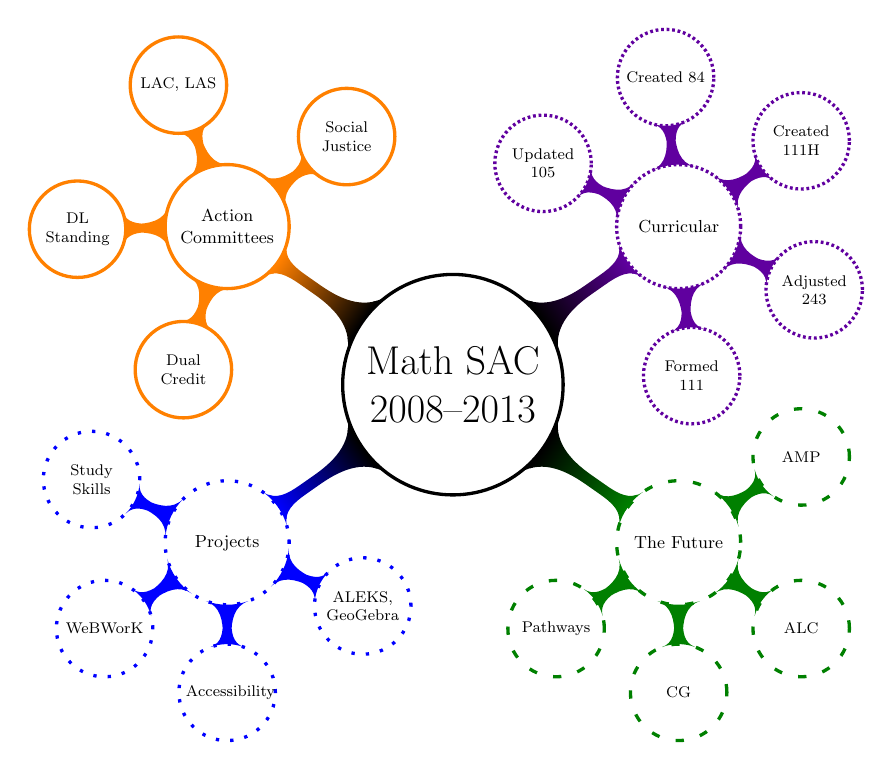
\begin{tikzpicture}[mindmap,
				concept/.append style={fill={none}},
				root concept/.style={concept color=blue},
				level 1 concept/.append style=
					{level distance = 35mm},
				level 2 concept/.append style=
					{level distance = 19mm},
				every node/.append style={align=center,scale=0.7},
			]
			\node [concept,font=\huge] {Math SAC\\2008--2013}
			child[grow=145, concept color=orange,visible on=<2->] {node[concept] {Action Committees}
					child[grow=37, visible on=<2->]{node[concept] {Social Justice}}
					child[grow=109, visible on=<2->]{node[concept] {LAC, LAS}}
					child[grow=181, visible on=<2->]{node[concept] {DL Standing}}
					child[grow=253, visible on=<2->]{node[concept] {Dual Credit}}
				}
			child[loosely dotted,concept color=blue,grow=215,visible on=<3->] {node[concept] {Projects}
					child[grow=155,visible on=<3->]{node[concept] {Study Skills}}
					child[grow=215,visible on=<3->]{node[concept] {WeBWorK}}
					child[grow=270,visible on=<3->]{node[concept] {Accessibility}}
					child[grow=335,visible on=<3->]{node[concept] {ALEKS, GeoGebra}}
				}
			child[dash pattern=on 1pt off 1pt on 1pt off 1pt, concept color=blue!50!purple,grow=35,visible on=<4->] {node[concept] {Curricular}
					child[grow=35,visible on=<4-> ] {node[concept] {Created 111H}}
					child[grow=95,visible on=<4->] {node[concept] {Created 84}}
					child[grow=155,visible on=<4->] {node[concept] {Updated 105}}
					child[grow=275,visible on=<4->] {node[concept] {Formed 111}}
					child[grow=335,visible on=<4->] {node[concept] {Adjusted 243}}
				}
			child[loosely dashed,concept color=green!50!black,grow=325,visible on=<5->] {node[concept] {The Future}
					child[grow=215,visible on=<4-> ] {node[concept] {Pathways}}
					child[grow=35,visible on=<4->] {node[concept] {AMP}}
					child[grow=270,visible on=<4->] {node[concept] {CG}}
					child[grow=-35,visible on=<4->] {node[concept] {ALC}}
				};
			%\node at (0,0) [inner sep=9mm,decorate,circle,decoration=
			%{text along path,text={Equally Effective Equally Effective Equally Effective Equally Effective }}] {};
		\end{tikzpicture}
	}
\end{frame}

%----------------------------------------------------------------------------------------------------------------------------------------------------------------

\begin{frame}{A Possible Future for Developmental Mathematics}
	\includegraphics[width=\textwidth]{graphics/pathwayDiagram.pdf}
	%*Every student in a given section of Math in Context I would also be enrolled in a common section of the CG course. The instructors of a given pair of courses would work in a collaborative fashion and ideally visit one another's classes, especially the first week.
	%Unlinked sections of the CG course would be offered for entry level DE mathematics students whose initial placement is `above' Math in Context I. Students who pass Math in Context I but not the attendant CG course might be required to retake the course.
\end{frame}
\end{document}
%----------------------------------------------------------------------------------------------------------------------------------------------------------------
% old stuff- should be savalgable if necessary

\begin{frame}{Highlights from the last 5 years}
	\begin{block}{Projects}
		\begin{itemize}
			\item Study Skills Workbook
			\item Mathematics Accessibility Study

			\item WeBWorK
			      \begin{itemize}
				      \item Accesibility
				      \item Free
				      \item Problem Library Development
				      \item Future Developments
			      \end{itemize}

			\item Other Technology innovations in the classroom
			      \begin{itemize}
				      \item ALEKS
				      \item GeoGebra
			      \end{itemize}


		\end{itemize}
	\end{block}
\end{frame}
%----------------------------------------------------------------------------------------------------------------------------------------------------------------

\begin{frame}{Highlights from the last 5 years}
	\begin{block}{College wide service and professional development}
		\begin{itemize}
			\item Multiple college wide committees (including several chairs)
			\item Conference attendance
			\item Memberships in professional organizations
			\item Improved Dual Credit relationships
		\end{itemize}
	\end{block}

	\begin{block}{Enrollment}
		\begin{itemize}
			\item Overall growth
			\item Even stronger in LDC courses
		\end{itemize}
	\end{block}

\end{frame}
%----------------------------------------------------------------------------------------------------------------------------------------------------------------

\begin{frame}{Highlights from the last 5 years}
	\begin{block}{Curricular changes}
		\begin{itemize}
			\item  Condensed MTH 111B and MTH 111C into MTH 111
			\item MTH 105 replaced MTH111A and increased enrollment
			\item MTH 111H
			\item All classes with MTH prefix are now part of the MTH SAC
			\item MTH 243 credit change and future pre-requisite change
			\item MTH 84 (\LaTeX)
			\item ALC (Alternative Learning Centers) %courses allow students the opportunity to work on the math they need to work on for credit (but not for pre-requisites).
			\item AMP (Accelerated Math Placement) %allows students to review material and gives them the chance to take the placement exam again for (possibly) higher placement.
		\end{itemize}
	\end{block}
\end{frame}
%----------------------------------------------------------------------------------------------------------------------------------------------------------------

\begin{frame}{The Future of DE}

	%insert flow chart here
	%maybe this will work once it gets compiled?

	%\makebox[\textwidth][c]{%
	%  \input{graphics/pathwayDiagram.tex}
	%  }

	\includegraphics[width=\textwidth]{graphics/pathwayDiagram.pdf}

	%*Every student in a given section of Math in Context I would also be enrolled in a common section of the CG course.  The instructors of a given pair of courses would work in a collaborative fashion and ideally visit one another's classes, especially the first week.

	%Unlinked sections of the CG course would be offered for entry level DE mathematics students whose initial placement is `above' Math in Context I.  Students who pass Math in Context I but not the attendant CG course might be required to retake the course.

\end{frame}
%----------------------------------------------------------------------------------------------------------------------------------------------------------------

\begin{frame}{Highlights from the last 5 years}
	\begin{block}{Curricular changes}
		\begin{itemize}
			\item Condensed MTH 111B and MTH 111C into MTH 111
			\item MTH 105 replaced MTH111A and increased enrollment
			\item MTH 111H
			\item All classes with MTH prefix are now part of the MTH SAC
			\item MTH 243 credit change and future pre-requisite change
			\item MTH 84 (\LaTeX)
			\item ALC (Alternative Learning Centers) %courses allow students the opportunity to work on the math they need to work on for credit (but not for pre-requisites).
			\item AMP (Accelerated Math Placement) %allows students to review material and gives them the chance to take the placement exam again for (possibly) higher placement.
		\end{itemize}
	\end{block}
\end{frame}


\end{document}

